Consideramos una cadena de $2N$ qubits \textit{transmon} acoplada a primeros vecinos, con condiciones periódicas de contorno (PBC).
\subsection{Hamiltoniano individual}
Cada transmon $j$ tiene hamiltoniano
\begin{equation}
    \hat H_j = 4E_C (\hat  n_j - n_j^0)^2 - E_J \cos \hat \phi_j \label{eq:single_transmon_hamiltonian}    
\end{equation}
con $\hat n_j$ y $\hat \phi_j$ variables canónicamente conjugadas
\begin{equation}
    \left[\hat \phi_j, \hat n_j\right] = i,
\end{equation}
y $n_j^0$ la carga de gate inducida por el entorno del transmon sobre él. Como se muestra en \cite{Koch2007}, es posible encontrar el espectro de forma analítica observando que en la representación de carga, \eqref{eq:single_transmon_hamiltonian} se reduce a la ecuación de Mathieu \cite{Meixner1980}, de donde se obtiene
\begin{equation}
    E_k = 4E_C \mathcal{M}_\mathcal{A}\left[(k+1)\%2 + 2(-1)^k n_j^0, -2E_J / E_C\right], \label{eq:mathieu_spectrum}
\end{equation}
con $\mathcal{M}_\mathcal{A}(r, q)$ el valor característico de Mathieu para las funciones pares.\\

En el límite transmon ($E_J \gg E_C$), se puede demostrar que el espectro es insensible a $n_j^0$ por lo cual lo fijamos en cero para los siguientes análisis. Además en este límite, la profundidad del potencial justifica expandirlo en serie y truncar a los órdenes más bajos. Por otro lado, el tratamiento más común en este régimen es pasar a la base de operadores
\begin{subequations}
    \begin{align}
        \hat \phi &= \left(\frac{2E_C}{E_J}\right)^{1/4}(\hat b^\dag_j + \hat b_j)\\
        \hat n_j &= \frac{i}{2}\left(\frac{E_J}{2E_C}\right)^{1/4}(\hat b^\dag_j - \hat b_j),
    \end{align}
\end{subequations}
que se demuestran que satisfacen las relaciones de conmutación bosónicas
\begin{equation}
    \left[\hat b_j, \hat b_j^\dag\right] = 1.
\end{equation}
En la figura \ref{fig:transmon_truncation} se comparan los autovalores obtenidos de forma analítica por \eqref{eq:mathieu_spectrum} con los obtenidos de forma numérica en la base de estos operadores truncando en un número $N$ finito de estados. Para ello, se utilizó la expresión de los elementos de matriz en esta base del operador desplazamiento $\mathcal D(\alpha) = e^{\alpha \hat b_j^\dag - \alpha^*\hat b_j}$
\begin{equation}
    \langle m | e^{\alpha \hat b_j^\dag - \alpha^*\hat b_j} | n \rangle =
        \begin{cases}
            \begin{aligned}
            & e^{-\frac{|\alpha|^2}{2}} \sqrt{\frac{n!}{m!}} \, (\alpha)^{m-n} \\
            & \times L_n^{(m-n)}(|\alpha|^2),
            \end{aligned} & m \ge n \\[1ex]
            \begin{aligned}
            & e^{-\frac{|\alpha|^2}{2}} \sqrt{\frac{m!}{n!}} \, (-\alpha^*)^{n-m} \\
            & \times L_m^{(n-m)}(|\alpha|^2),
            \end{aligned} & m < n
        \end{cases},
\end{equation}
con $L_n^{(k)}$ los polinomios asociados de Laguerre \cite{walls2008Quantum}. Entonces el potencial puede expresarse como $\cos \hat \phi_j = \frac{1}{2}\left(\mathcal D(i\phi_{\text{0}}) + \mathcal D(-i\phi_{\text{0}})\right)$ con $\phi_0 = \sqrt[4]{2E_C / E_J}$.
\begin{figure}[t]
    \centering
    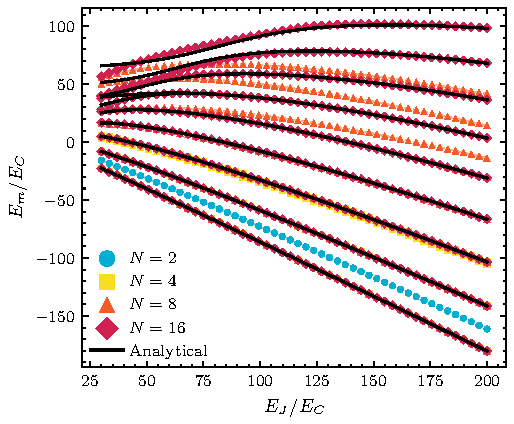
\includegraphics[width=0.75\columnwidth]{../../figures/export/single_transmon_truncation_final.pdf}%
    \caption{Comparación para distintos truncamientos de los primeros 9 niveles del hamiltoniano \eqref{eq:single_transmon_hamiltonian} en función del truncamiento en la base de operadores $b_j$, $b^\dag_j$. En línea negra se muestra el espectro obtenido de forma analítica usando la ecuación \eqref{eq:mathieu_spectrum}.}
    \label{fig:transmon_truncation}
\end{figure}
Expandiendo el potencial a orden 4 en $\hat \phi_j$ obtenemos la siguiente expresión
\begin{equation}
    \hat H_j \approx \underbrace{\hbar \omega_q \hat b^\dag_j \hat b_j}_{\text{Armónico}} - U\left[\underbrace{(\hat b_j)^2 + (\hat b_j^\dag)^2}_{\text{Pairing / Squeezing}} + \underbrace{(\hat b_j^\dag)^2(\hat b_j)^2}_{\text{Kerr}}\right]\label{eq:hamiltonian_comparison}
\end{equation}
donde nos quedamos con los términos de orden cuadrático y con el término de interacción que da una no linealidad de Kerr y se definieron $\hbar \omega_q = \sqrt{8E_CE_J} - E_C$ y $U = \frac{E_C}{2}$. En la figura \ref{fig:transmon_hamiltonian_comparison} se comparan los espectros obtenidos utilizando distintas versiones de \eqref{eq:hamiltonian_comparison} añadiendo una a una las contribuciones de cada término.
\begin{figure}[t]
    \centering
    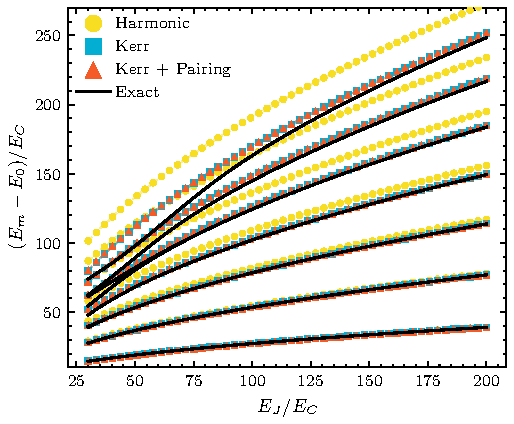
\includegraphics[width=0.75\columnwidth]{../../figures/export/single_transmon_hamiltonian_comparison.pdf}%
    \caption{Comparación de los primeros 7 niveles de un solo transmon empleando distintos términos de \eqref{eq:hamiltonian_comparison} para distintos valores de $E_J / E_C$.}
    \label{fig:transmon_hamiltonian_comparison}
\end{figure}
De la figura concluimos los siguientes puntos
\begin{itemize}
    \item Los primeros niveles se ven bien descritos usando la parte armónica del hamiltoniano
    \item El efecto del término Kerr domina por sobre el del término de squeezing
    \item Para niveles con $n\geq 3$ hace falta considerar el efecto de las interacciones
    \item La aproximación mejora conforme aumenta $E_J / E_C$
\end{itemize}
En general se puede quitar los términos de squeezing por medio de una transformación unitaria squeeze $\hat S_j(z) = \operatorname{exp}\left(\frac{1}{2}(z^* \hat b_j^2 - z \hat b_j^{\dag2})\right)$ con la cual los operadores transforman 
\begin{subequations}
\begin{align}
    \hat S_j^\dag(z) \hat b_j \hat S_j(z) &= \cosh(\abs{z})\hat b_j -\frac{z}{\abs{z}}\sinh(\abs{z})\hat b^\dag_j\\
    \hat S_j^\dag(z) \hat b_j^\dag \hat S_j(z) &= \cosh(\abs{z})\hat b_j^\dag -\frac{z^*}{\abs{z}}\sinh(\abs{z})\hat b_j
\end{align}\label{eq:squeeze_transformations}
\end{subequations}
% donde se encuentra que el parámetro de squeezing real dado por $\tanh(z) = \frac{U}{\hbar \omega_q}$ tiene el efecto de eliminar esos términos y renormalizar la frecuencia de la parte armónica $\hbar \omega_q \rightarrow \sqrt{(\hbar \omega_q)^2 - U^2}$.

Al realizar la transformación y descartando los términos de ordenes superiores que no conservan el número de excitaciones, se puede llegar a un hamiltoniano que posee solo la parte armónica y Kerr con $\hbar \omega_q$, $U$ ligeramente renormalizados. Dicha renormalización es muy pequeña así que por el momento la dejamos de lado.  Concluimos que modelamos cada transmon simplemente como un oscilador armónico con una no linealidad de Kerr negativa.\\

\subsection{Acoplamiento a primeros vecinos}
Ahora consideramos una cadena SSH de transmons acoplada a primeros vecinos por capacitores y por SQUIDs simétricos como se muestra en la figura \ref{fig:transmon_chain}. Consideramos que el sistema está compuesto por $N$ celdas unidad de dos qubit. El hamiltoniano de este sistema está dado por
\begin{equation}
    \hat H = \hbar \omega_c \hat a^\dag \hat a + \sum_{j,\, \sigma} \hat H_{j, \, \sigma} + \sum_{j} \left(\hat H_{j}^{(AB)} + \hat H_{j}^{(j+1)}\right)
\end{equation}
con $\sigma = A, \, B$ indicando la subred y $\hat H_j^{AB}$, $\hat H_j^{j+1}$ los hamiltonianos de acoplamiento intra e intercelda respectivamente. Obviando por el momento la dependencia de las constantes de acoplamiento con los parámetros del circuito, tenemos que
\begin{subequations}
    \begin{align}
        \hat H_j^{AB} &= -\hbar g_{1}(\hat b^\dag_{j, A} - \hat b_{j, A})(\hat b^\dag_{j, B} - \hat b_{j, B}) \nonumber\\
                      &\quad - E_{J, 1}(\hat \Phi^{(AB)}_{\text{ext}})\cos(\hat \phi_{j, B} - \hat \phi_{j, A})\\
        \hat H_j^{j+1} &= -\hbar g_{2}(\hat b^\dag_{j, B} - \hat b_{j, B})(\hat b^\dag_{j+1, A} - \hat b_{j+1, A}) \nonumber\\
                       &\quad - E_{J, 2}(\hat \Phi^{(j+1)}_{\text{ext}})\cos(\hat \phi_{j+1, A} - \hat \phi_{j, B})
    \end{align}
\end{subequations}
Donde
\begin{equation}
    E_{J,\, x}(\hat \Phi_{\text{ext}}) = 2E_{J,\, x}^0\cos(\hat \Phi_{\text{ext}}),\quad (x=1,\, 2)
\end{equation}
es la energía Josephson del SQUID en función de la energía Josephson de cada juntura que la conforma $E_{J,\, x}^0$ y el flujo externo que lo atraviesa $\hat \Phi_{\text{ext}}$. Abrimos la posibilidad de que el flujo magnético a través de cada SQUID pueda estar en el régimen cuántico. En nuestro caso particular, consideraremos que el flujo externo tiene una componente constante $\Phi_{\text{DC}}$ común a todo el circuito y otra dada por las fluctuaciones de flujo de un resonador microondas cercano, entonces
\begin{subequations}
    \begin{align}
        \hat \Phi^{(AB)}_{\text{ext}}&= \Phi_{\text{DC}} + \gamma_1 (\hat a^\dag + \hat a)\\
        \hat \Phi^{(j+1)}_{\text{ext}}&= \Phi_{\text{DC}} + \gamma_2 (\hat a^\dag + \hat a),
    \end{align}
\end{subequations}
Donde tomamos la convención $\gamma_1, \equiv \gamma$ con $\gamma > 0$ y $\gamma_2 = \pm \gamma_1$. Esta convención surge de considerar dos situaciones que se muestran en la figura \ref{fig:SQUID_placing}:
\begin{enumerate}
    \item Usamos un resonador microondas \textit{lumped element} y el flujo en todos los SQUIDs es homogéneo
    \item Usamos un resonador microondas distribuido y colocamos cada SQUID en antinodos opuestos consecutivos
\end{enumerate}
Para maximizar el efecto de dichas fluctuaciones, usamos $\Phi_{\text{DC}} = \pi/2$. Finalmente, aprovechando el régimen transmon, expandimos el término de interacción obteniendo
\begin{equation}
    \cos(\hat \phi_1 - \hat \phi_2) \approx 1 + \hat \phi_1 \hat \phi_2 - \frac{1}{2}(\hat \phi_1^2 + \hat \phi_2^2)
\end{equation}
por lo cual definiendo $\hbar g_{J,\,1} \equiv 2E_{J,\,1}^0\phi_0^2$, $\hbar g_{J, \, 2} \equiv \text{sgn}(\gamma_2) 2E_{J, \, 2}^0 \phi_0^2$ llegamos a la expresión
\begin{equation}
    \hat H = \hbar \omega_c \hat a^\dag \hat a + \hat H_C 
                - \sin\!\left(\gamma(\hat a^\dag + \hat a)\right) \hat H_J
\end{equation}
donde se definieron los hamiltonianos capacitivo y Josephson: 
\begin{subequations}
    \begin{align}
        \hat H_C &= \sum_{j, \sigma} \hbar \omega_q \hat b^\dag_{j\sigma} \hat b_{j\sigma} - U\hat b^\dag_{j\sigma}\hat b^\dag_{j\sigma}\hat b_{j\sigma}\hat b_{j\sigma}\nonumber\\
                &\quad+ \sum_j \left(\hbar g_{C,1}\hat b^\dag_{j,A}\hat b_{j,B} + \hbar g_{C,2}\hat b^\dag_{j,B} \hat b_{j+1,A} +\text{h.c.}\right)\nonumber\\ 
               &\quad-\sum_j \left(\hbar g_{C,1}\hat b^\dag_{j,A}\hat b^\dag_{j,B} + \hbar g_{C,2}\hat b^\dag_{j,B} \hat b^\dag_{j+1,A}+\text{h.c.} \right) \\
        %
        \hat H_J &= \hbar(g_{J,1} + g_{J,2})\sum_{j,\sigma}  
                \hat b^\dag_{j,\sigma}\hat b_{j,\sigma} 
                - \frac{1}{2}\left(\hat b^{\dag 2}_{j,\sigma} + \text{h.c.}\right) \nonumber\\
               &\quad - \sum_j \left(\hbar g_{J,1}\hat b^\dag_{j,A}\hat b_{j,B} 
                + \hbar g_{J,2}\hat b^\dag_{j,B} \hat b_{j+1,A} + \text{h.c.}\right) \nonumber\\
               &\quad - \sum_j \left(\hbar g_{J,1}\hat b^\dag_{j,A}\hat b^\dag_{j,B} 
                + \hbar g_{J,2}\hat b^\dag_{j,B} \hat b^\dag_{j+1,A} + \text{h.c.}\right) + \delta_J \label{eq:Josephson_H_real}
    \end{align}\label{eq:real_space_hamiltonians}
\end{subequations}
Con $\delta_J = -2(E_{J,\,1}^0 + \operatorname{sgn}(\gamma_2)E_{J,\,2}^0)(1-\frac{\phi_0^2}{4})$. Observar que en el caso $E_{J,\,1}^0 = E_{J,\,2}^0$, $\gamma_2 < 0$, en \eqref{eq:Josephson_H_real} solo sobreviven los términos que mezclan el pseudospin $\sigma$. Usualmente los términos de squeezing a dos modos $\hat b^\dag_{j} \hat b^\dag_{j+1}$, $\hat b_{j} \hat b_{j+1}$ suelen ser ignorados debido a que los qubits son tratados en el límite de acople capacitivo débil y por tanto es posible usar la aproximación de onda rotante (RWA) para descartar su efecto. Sin embargo, queremos llegar al límite de acoplamiento fuerte haciendo $g_{C,1}, g_{C,2} \lesssim \hbar \omega_q$, por lo cual consideramos los efectos de estos términos en los próximos tratamientos. Por otra parte, se puede apreciar que los hamiltonianos \eqref{eq:real_space_hamiltonians} son una realización de la cadena de Kitaev bosónica en formato SSH \cite{McDonald2018}. Finalmente, se puede demostrar que $\gamma = \frac{M\Phi_{\text{zpf}}}{L\Phi_0}$, con $M$ la inductancia mutua entre el resonador y cada SQUID, $L$ la inductancia propia del resonador, $\Phi_{\text{zpf}}$ la amplitud de fluctuaciones de punto cero del resonador y $\Phi_0$ el cuanto de flujo superconductor. Para los valores de inductancia mutua posibles en un circuito, se puede encontrar que $\gamma  \ll 1$ por lo cual, en la gran mayoría de próximos análisis nos enfocaremos en la aproximación $\sin(\gamma(\hat a^\dag + \hat a)) \approx \gamma(\hat a^\dag + \hat a)$.